\subsection{Trigonometry}
\fbox{\begin{minipage}{0.31\textwidth}
\begin{align*}
& \sin(v+w)=\sin v\cos w+\cos v\sin w\\
& \sin(v-w)=\sin v\cos w-\cos v\sin w\\
& \tan(v+w)=\tfrac{\tan v+\tan w}{1-\tan v\tan w}\\
& \sin v+\sin w=2\sin\tfrac{v+w}{2}\cos\tfrac{v-w}{2}\\
& \cos v+\cos w=2\cos\tfrac{v+w}{2}\cos\tfrac{v-w}{2}
\end{align*}
\end{minipage}}


\subsection{Ball}
\fbox{\noindent\begin{minipage}{0.12\textwidth}\raggedleft
$a = \sqrt{h * (2R - h)}$\\ 
$V = \pi * h^2(R -\frac{h}{3})$
\end{minipage}}
\hfill
\fbox{\begin{minipage}{0.08\textwidth}
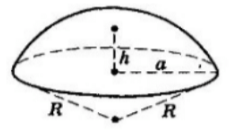
\includegraphics[width=\textwidth]{content/various/ball-segment.png}
\end{minipage}}

\fbox{\noindent\begin{minipage}{0.17\textwidth}\raggedleft
$V = \frac{1}{6}\pi h(3a^2+3b^2+h^2)$\\
$R = \sqrt{\frac{((a - b)^2 + h^2)((a + b)^2 + h^2)}{4h^2}}$
\end{minipage}}
\hfill
\fbox{\begin{minipage}{0.08\textwidth}
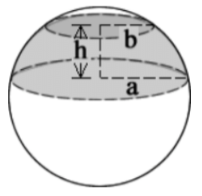
\includegraphics[width=\textwidth]{content/various/ball-layer.png}
\end{minipage}}

\subsection{Pick's theorem}
Suppose that a polygon has integer coordinates for all of its vertices. 
Let $i$ be the number of integer points inside, and let $b$ be the number of integer points on boundary. 
Then the area $S = i + \tfrac{b}{2} - 1$.

\subsection{Ptolemy's theorem}
If the cyclic quadrilateral is $ABCD$, then
$AC \cdot BD = AB \cdot CD + AD \cdot BC$.

\subsection{Ceva's theorem}
Given a triangle $\triangle ABC$ with a point $P$ inside the triangle,
continue lines $AP$, $BP$, $CP$ to hit $BC$, $CA$, $AB$ at $D$, $E$, $F$,
respectively.
Ceva's theorem states that
$\frac{AF}{FB} \cdot \frac{BD}{DC} \cdot \frac{CE}{EA} = 1$. 

\subsection{Simson line}
Given a triangle $\triangle ABC$ and a point $P$ on its circumcircle,
the three closest points to $P$ on lines $AB$, $AC$, and $BC$ are collinear.
The line through these points is the Simson line of $P$.

\subsection{Euler line}
The line on which the orthocenter, triangle centroid, circumcenter,
and a number of other important triangle centers lie. 

\subsection{Platonic solids}
\begin{tabular}{ |c|c|c|c| } 
\hline
Polyhedron & Vertices & Edges & Faces \\ 
\hline
tetrahedron & 4 & 6 & 4 \\ 
\hline
cube & 8 & 12 & 6 \\ 
\hline
octahedron & 6 & 12 & 8 \\
\hline
dodecahedron & 20 & 30 & 12 \\
\hline
icosahedron & 12 & 30 & 20 \\
\hline
\end{tabular}
 
